\newpage

\section{Social Events}

An important aspect of a conference like GUADEC is to meet in a less formal
environment and make new friends in the community. We plan to host multiple
social events for everyone to attend, if at all possible we will try to
provide free drinks or even free food at some of the events.

\begin{multicols}{2}
\raggedcolumns

\subsection{AKK/Z10 Beer Event}

With the AKK and Z10 we have two non-profits run by the student community that
maintain bars close to the University (KIT South Campus).
Both of these locations are ideal as they are kept by volunteers and with just
a couple of volunteers of our own and relatively little money we can
serve drinks to all conference attendees free of charge all night long.

\subsection{Football and Games}

It is customary for GUADEC to host a football game on one of the evenings. We will
rent a football field. By working together with a student organization at the
KIT we can rent one on the university campus free of charge.

\subsection{Picnic}

Karlsruhe has a nice park to the north of the castle which provides a beautiful
place to play games and enjoy the day. One one evening we would like to do
a picnic in this park.

\columnbreak

\begin{tikzpicture}
  \node[outer sep=0,inner sep=0] (img) {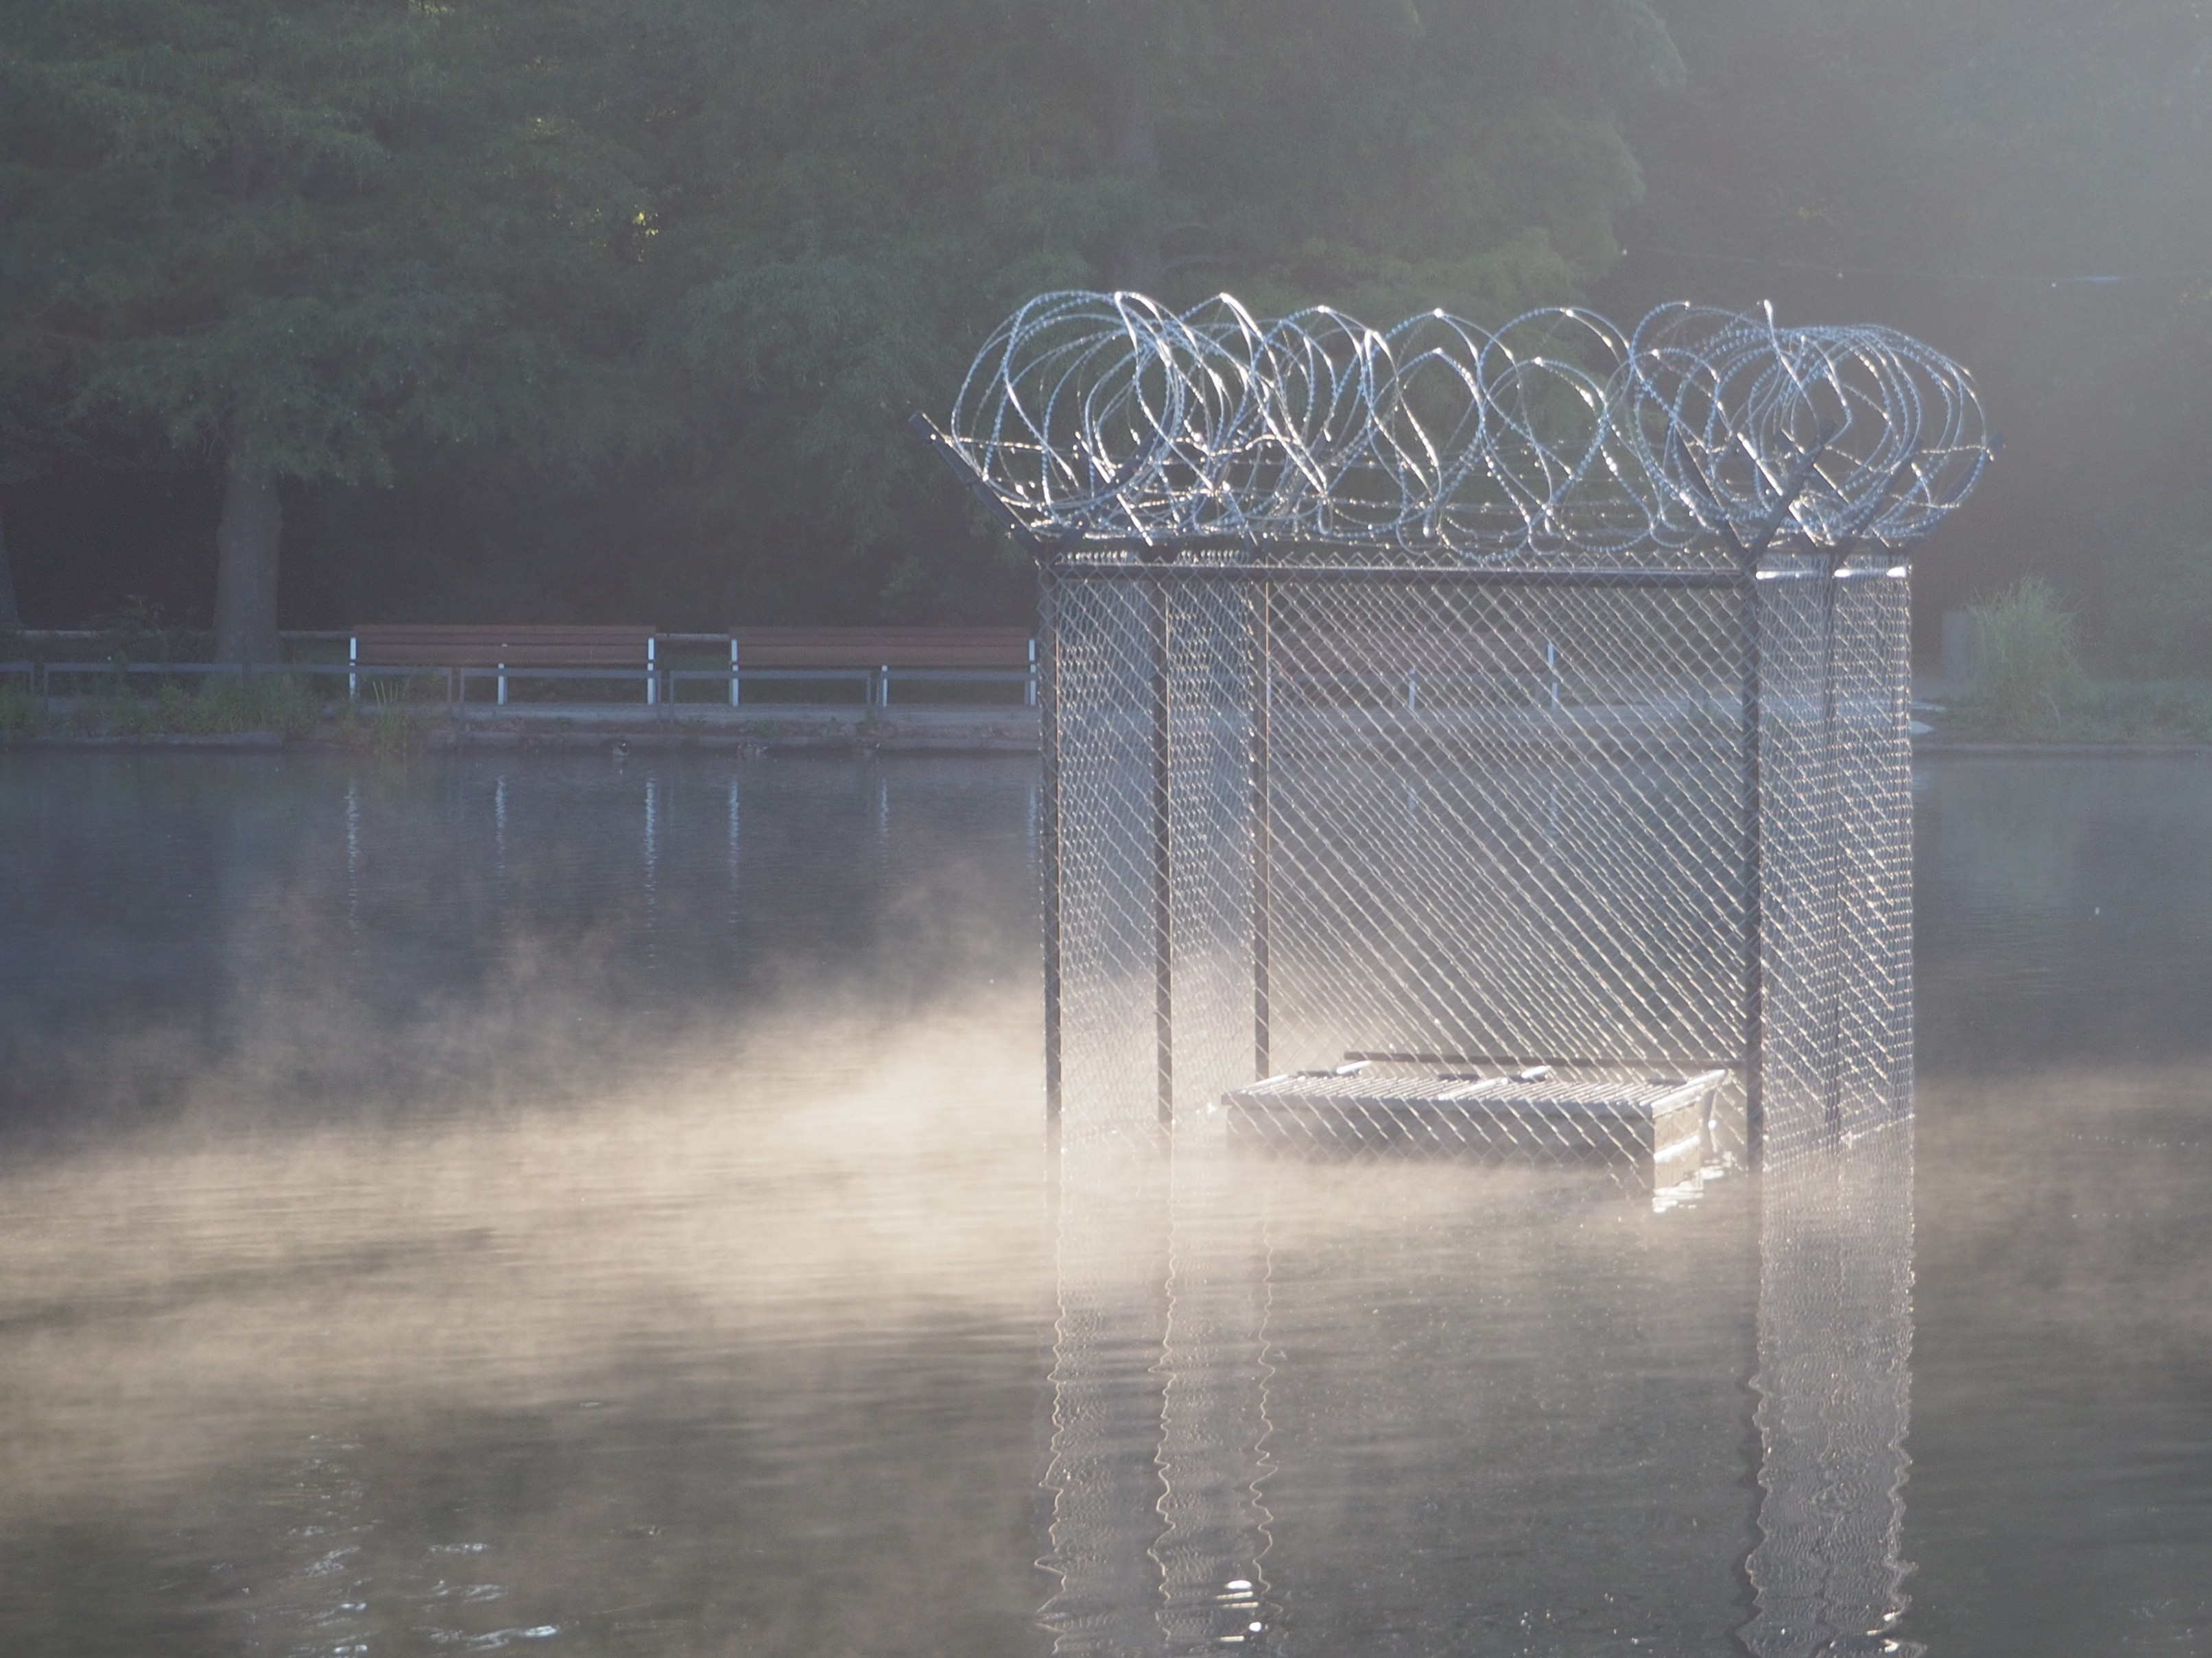
\includegraphics[width=\linewidth]{images/city/art-1.jpg}};
  \node[anchor=south west,color=white,outer sep=1ex] at (img.south west) {\imgtitle{Photo by Benjamin Berg}{Art installation, ZKM}{CC BY-SA 4.0}{}};
\end{tikzpicture}

\subsection{Barbecue}

On the first evening we are planning to barbecue. We can provide attendees with
food and drinks throughout the evening as they are arriving in Karlsruhe.

\subsection{Center for Art and Media (ZKM)}

The ZKM\footnote{Zentrum für Kunst und Medien} the Center for Art and Media is
a world renowned museum in Karlsruhe and even one of our possible venues
(see also section~\ref{zkm-venue}). We can recommend anyone visiting to
Karlsruhe to spend a couple of hours in this museum, so we plan to book a tour
of this museum for everyone interested.



\end{multicols}

\newpage
